\chapter{Code4Code} %\label{1cap:spinta_laterale}
% [titolo ridotto se non ci dovesse stare] {titolo completo}
%

\begin{citazione}
La piattaforma \textsc{Code4Code} non è stata implementata interamente, ma solo nella parte relativa all'Intelligenza Artificiale. Nonostante ciò l'idea della piattaforma è concreta ed il messaggio che vuole comunicare è chiaro e preciso e per farlo sono necessari vari strumenti che sono stati ideati e dei quali si ha una parziale idea di implementazione. In questo capitolo vengono ripetuti gli obiettivi della piattaforma mediante una panoramica generale della stessa e vengono presentate le funzionalità principali che assolvono allo scopo di supportare la collaborazione tra gli utenti. È presente un breve workflow dell'utilizzo della piattaforma che chiarisce il modo in cui gli strumenti di Intelligenza Artificiale presentati nei precedenti capitoli vengono utilizzati nel momento in cui l'utente usufruisce della piattaforma. Il capitolo si conclude con la trattazione di aspetti relativi all'architettura del sistema e ai Framework utilizzati.
\end{citazione}
\newpage

\section{Funzionalità della piattaforma} %\label{1sec:scopo}
Seppur implementata solo nella parte relativa all'Intelligenza Artificiale, la piattaforma \textsc{Code4Code} è stata ideata per assolvere ad un certo compito e per avere determinate funzionalità. Come specificato nei precedenti capitoli, la piattaforma \textsc{Code4Code} si basa su uno scambio reciproco di conoscenze tra gli utenti facendo sì che non vi sia necessità di scambi di denaro. In altri termini, se l’utente \emph{A} desidera imparare una certa tecnologia \emph{X} non deve disporre di una somma di denaro da offrire all’utente \emph{B} che gli insegna ad usare quella tecnologia, in quanto l’utente \emph{B} avrà bisogno di imparare una tecnologia \emph{Y} che \emph{A} potrà insegnargli.
I punti focali dell’applicazione risultano essere, dunque, la comunicazione e il matching tra i diversi utenti che deve avvenire secondo parametri ben precisi, oltre che gli strumenti di supporto che la piattaforma stessa deve fornire agli utenti per l’apprendimento. Per comprendere la rilevanza di questi fattori è conveniente seguire il workflow dell’utente registrato all’applicazione (verranno saltati i passaggi relativi alla registrazione e all’autenticazione in quanto sono passaggi "classici").
Dopo che l’utente effettua la registrazione e fa il Log In per la prima volta viene sottoposto ad alcune semplici domande inerenti al mondo della programmazione che verranno usate per "conoscerlo meglio" e per comprendere le sue esigenze e quello che ha da offrire agli altri utenti della piattaforma. La figura \ref{fig:linguaggi_padroneggiati} mostra l'interfaccia utente per l'inserimento dei Linguaggi padroneggiati, mentre la figura \ref{fig:frameworks_padroneggiati} mostra l'interfaccia per l'inserimento dei Frameworks e delle Librerie padroneggiate. 
\begin{figure}[!htb]
    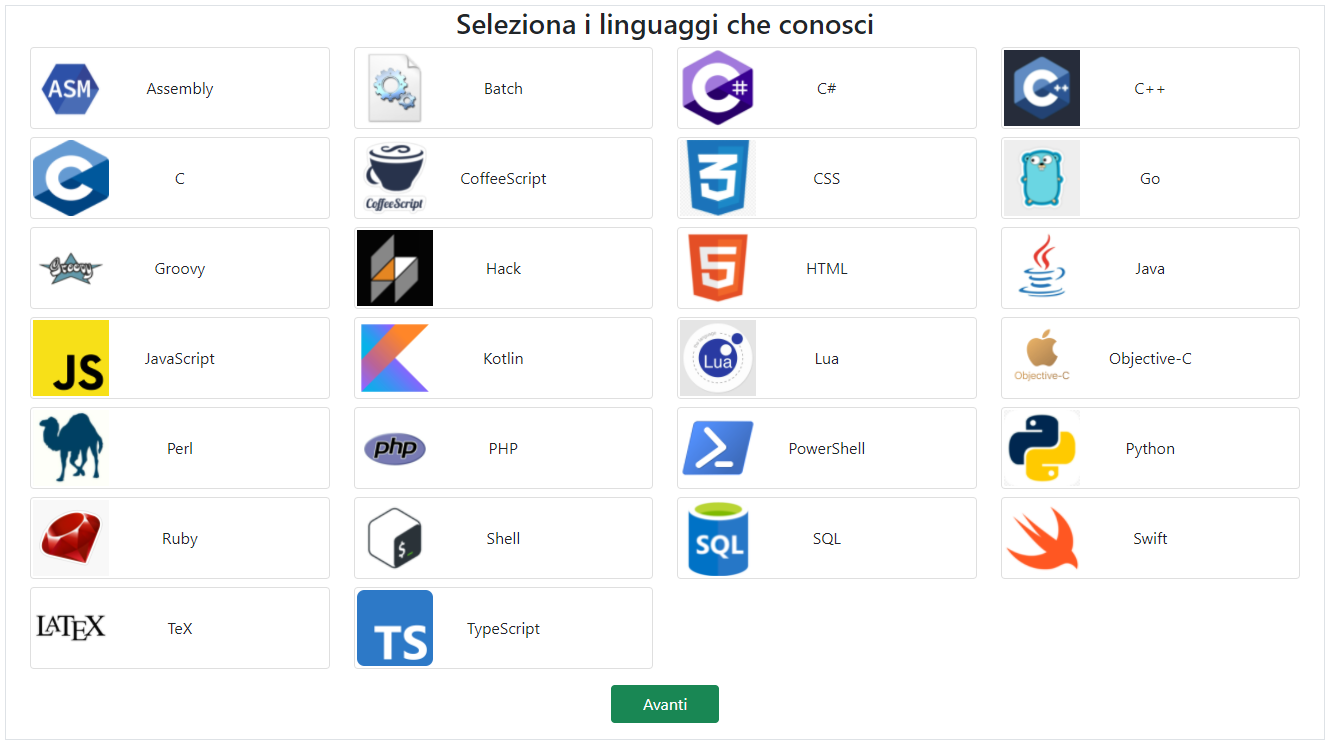
\includegraphics[width=\textwidth]{capitoli/images/linguaggi_padroneggiati.png}
    \caption{Form per l'inserimento dei Linguaggi padroneggiati dall'utente}
    \label{fig:linguaggi_padroneggiati}
\end{figure}
\begin{figure}[!htb]
    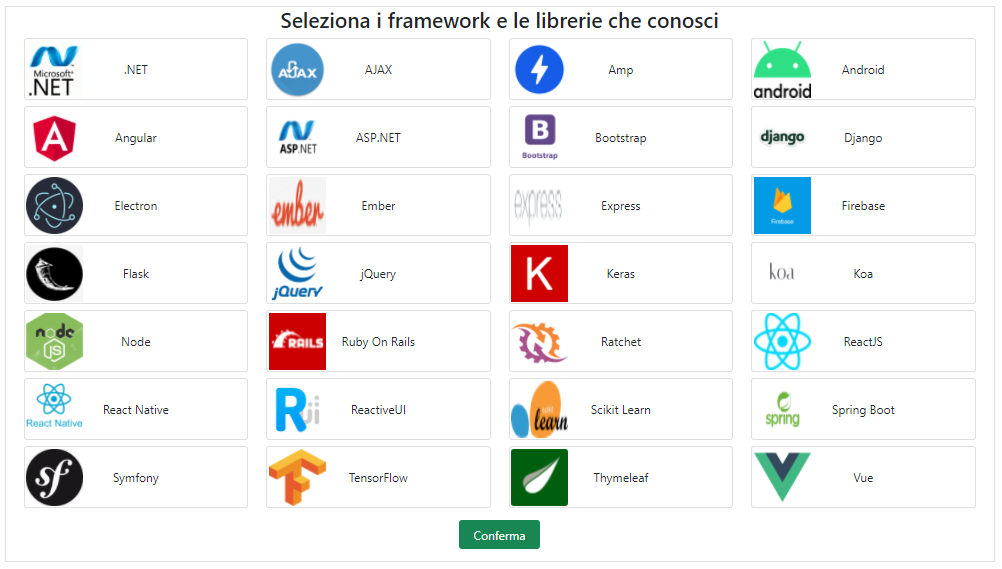
\includegraphics[width=\textwidth]{capitoli/images/frameworks_padroneggiati.png}
    \caption{Form per l'inserimento dei Frameworks e delle Librerie padroneggiate dall'utente}
    \label{fig:frameworks_padroneggiati}
\end{figure}
\\È possibile evitare che l'utente debba inserire manualmente le tecnologie che conosce, dandogli la possibilità di effettuare il Log In con \emph{GitHub} e chiedendogli di concedere l'autorizzazione alla lettura delle sue Repositories pubbliche e private. In questo modo è possibile prelevare i dati relativi alle tecnologie utilizzate nelle sue Repositories. A tal proposito è necessario fare due precisazioni:
\begin{itemize}
    \item In primo luogo ottenere le tecnologie utilizzate nella Repositories significa ottenere i Linguaggi, i Frameworks e le Librerie. I Linguaggi sono facilmente ottenibili grazie alle \emph{API} pubbliche messe a disposizione da \emph{GitHub} (un semplice modulo che effettua tale tipo di lavoro è stato facilmente implementato), mentre per quanto riguarda i Frameworks e le Librerie ci si affiderà ai tag delle Repositories (che non sempre contengono questo tipo di informazioni) e verranno utilizzate opportune tecniche per ricondurre il nome del tag al nome del Framework o della Libreria corrispondente, eventualmente andando ad utilizzare tecniche simili o del tutto equivalenti a quelle di \emph{NLP} presentate nel precedente capitolo.
    \item Il fatto che una determinata tecnologia sia presente in una Repository di cui l'utente risulta essere contributor, non significa necessariamente che l'utente padroneggi quella tecnologia; per tale ragione è opportuno che le tecnologie prelevate da \emph{GitHub} vengano proposte all'utente e che gli venga, dunque, data la possibilità di modificarle opportunamente.
\end{itemize}
Giunti a questo punto, la piattaforma suggerisce all'utente un insieme di Linguaggi, Frameworks e Librerie consigliati utilizzando le metodologie trattate nel capitolo precedente, come illustrato nella figura \ref{fig:tecnologie_suggerite}.
\begin{figure}[!htb]
    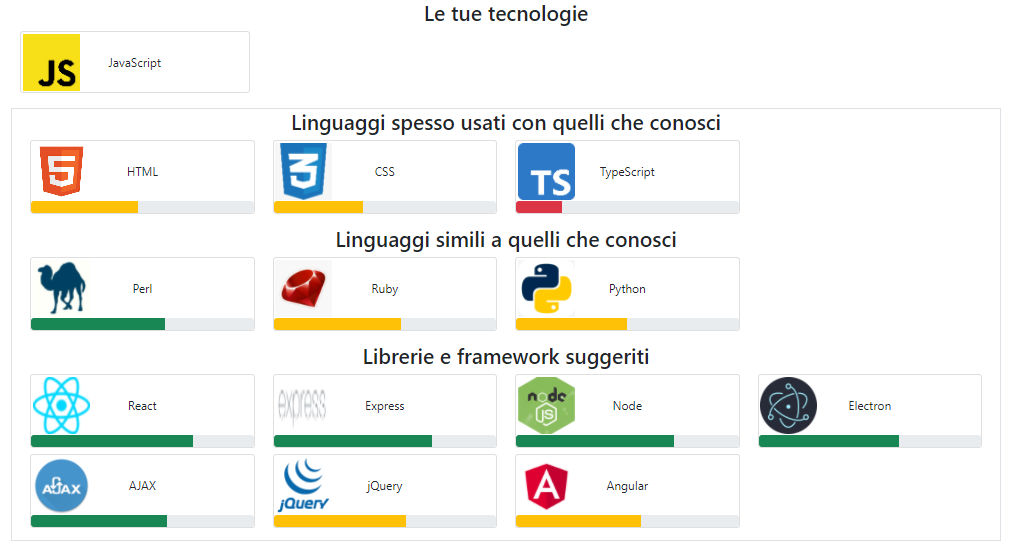
\includegraphics[width=\textwidth]{capitoli/images/tecnologie_suggerite.png}
    \caption{Risultato dell'Algoritmo che suggerisce Tecnologie Software}
    \label{fig:tecnologie_suggerite}
\end{figure}
\\L'utente può scegliere una o più tecnologie da imparare e la piattaforma provvederà a suggerirgli un insieme di utenti con cui iniziare una collaborazione mediante un algoritmo di Intelligenza Artificiale di cui è stato fornito un accenno di progettazione nel capitolo precedente. Due utenti si mettono in contatto tramite una richiesta di collaborazione che potrà essere effettuata solo se l’utente destinatario della richiesta padroneggia almeno una tecnologia che l’utente mittente vuole imparare e vuole imparare almeno una tecnologia padroneggiata dall’utente mittente. Se l’utente destinatario accetterà la richiesta, si creerà una collaborazione tra i due utenti; a questo punto la piattaforma deve fornire un insieme di strumenti che consentono ai due utenti di collaborare in maniera agevole ed efficiente. 
Di seguito verranno proposte e descritte diverse funzionalità:
\begin{itemize}
    \item Dovrebbe essere previsto un sistema di chat immediato che consenta agli utenti di comunicare in tempo reale per accordarsi sulle sessioni di "apprendimento"
    \item Le sessioni di apprendimento dovrebbero avvenire tramite lezioni in tempo reale, svolte mediante chiamate o videochiamate, in cui sia possibile condividere lo schermo per far sì che l’utente che insegna possa mostrare in tempo reale il codice che scrive e l’esecuzione dello stesso. Tali lezioni dovrebbero essere schedulate e la piattaforma dovrebbe tenere traccia dello schedule stesso mediante un calendario, che possa essere usato sia per tracciare lo schedule delle lezioni, che per aggiungerne di nuove. Un utente può aggiungere una lezione in cui lui sarà insegnante, potrà scegliere l’allievo e la tecnologia da insegnare e la lezione aggiunta verrà subito mostrata sul calendario dell'utente allievo. (figura \ref{fig:calendario}).
    \begin{figure}[!ht]
        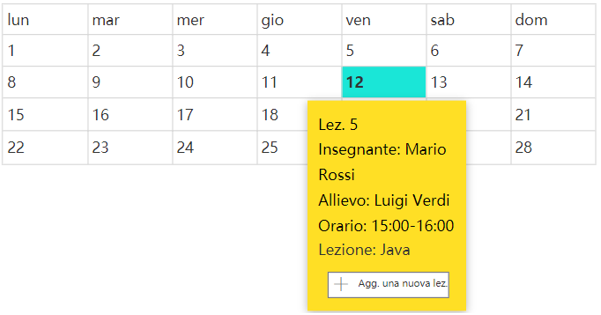
\includegraphics[width=\textwidth]{capitoli/images/calendario.png}
        \caption{Mockup del calendario che tiene traccia degli schedule delle lezioni}
        \label{fig:calendario}
    \end{figure}
    \item Il miglior modo per imparare è "provare sul campo", quindi dopo le sessioni di apprendimento è necessario che l’utente che sta imparando provi praticamente quanto ha appreso durante le lezioni. A tale scopo la piattaforma deve mettere a disposizione un sistema di assegnamento di task tramite il quale l’utente che sta insegnando può assegnare uno o più task all’utente che sta imparando. Il tutto potrebbe essere semplificato tramite un’integrazione con \emph{GitHub}, in modo tale che la piattaforma tenga traccia dei task (testo dell’esercizio), di un eventuale schedule dei task (tramite un calendario) e del link alla Repository di \emph{GitHub} contenente una proposta di soluzione svolta dall’utente che sta imparando, che verrà poi corretta dall’utente che insegna.
\end{itemize}
È importante sottolineare che i ruoli di "utente che insegna" e di "utente che impara" sono assolutamente dinamici in quanto nell’ambito di diversi meeting questi due ruoli potrebbero invertirsi (idealmente vi sarà un numero di meeting in cui l’utente A è insegnante e B è allievo, uguale al numero di meeting in cui l’utente A è allievo e B è insegnante). 
\section{Architettura del sistema} %\label{1sec:scopo}
La piattaforma \textsc{Code4Code} si concretizza in una \emph{WebApp} fruibile mediante un semplice Web Browser. Vi è un \emph{Web Server} scritto in \emph{Java} che serve le richieste del Client mediante delle \emph{REST API}. Durante l'utilizzo della piattaforma si interagisce con tre ulteriori Server:
\begin{itemize}
    \item Il primo Server, scritto in \emph{Python}, fornisce i risultati del modulo di Intelligenza Artificiale che suggerisce Frameworks e Librerie all'utente.  
    \item Il secondo Server è quello di \emph{Mattermost} \cite{mattermost}, strumento pensato per risolvere il problema delle chiamate e delle videochiamate con condivisione schermo. \emph{Mattermost} è una piattaforma \emph{open source} e \emph{self-hosted} a sé stante, ideata per la collaborazione nell'ambito di un'organizzazione e che fornisce servizi di chat in tempo reale con tanto di condivisione di file, chiamate, videochiamate, creazione di canali di comunicazione, funzionalità di condivisione schermo, il tutto accessibile mediante Web Browser come il resto delle funzionalità della piattaforma \textsc{Code4Code}. Dal momento che \emph{Mattermost} è \emph{open source}, è possibile ricompilare i sorgenti per modificare sia il \emph{Front-End} che il \emph{Back-End} della piattaforma al fine di adattarla ulteriormente al contesto di utilizzo evitando gli utilizzi impropri e decontestualizzati da parte dell'utente.
    \item Il terzo Server è il \emph{DataBase Server} che mediante un apposito \emph{DBMS} gestisce le entità persistenti della piattaforma.
\end{itemize} 
\begin{figure}[!htb]
    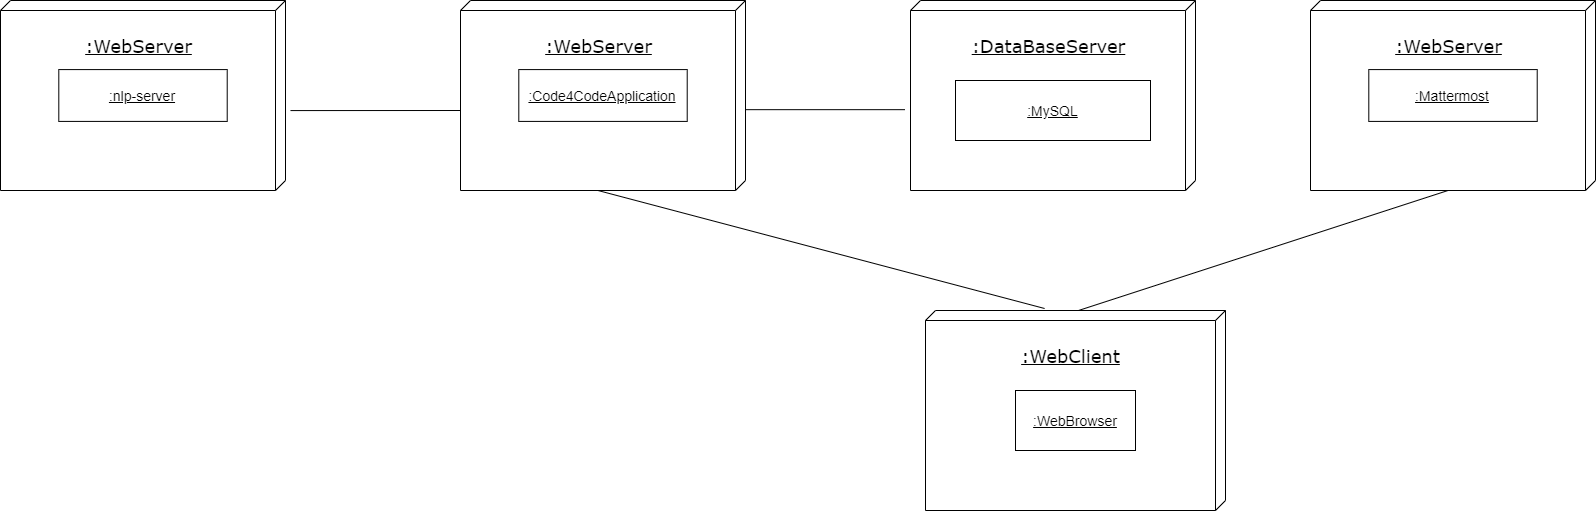
\includegraphics[width=\textwidth, height=6cm]{capitoli/images/progettazione_c4c.png}
    \caption{Architettura della piattaforma \textsc{Code4Code}}
    \label{fig:progettazione_c4c}
\end{figure}
\section{Framework utilizzati}
Per la realizzazione della piattaforma \textsc{Code4Code} sono stati impiegati vari Frameworks e Librerie. 
\begin{itemize}
    \item Per il \emph{Web Server} in \emph{Java} è stato utilizzato \emph{Spring} che ha reso agevole e veloce lo sviluppo delle \emph{REST API} implementate. Inoltre è stato utilizzato il motore di template \emph{Thymeleaf} per uno sviluppo moderno delle pagine \emph{HTML}, la cui parte grafica è stata facilmente curata grazie al Framework \emph{Bootstrap}.
    \item Per la parte di \emph{Natural Language Processing} in \emph{Python} è stata usata la Libreria \emph{Gensim} che ha fornito un'implementazione dell'algoritmo \emph{Word2Vec} per l'addestramento della Rete Neurale.
    \item Per le \emph{Association Rules}, utilizzate per il suggerimento dei Linguaggi, è stata utilizzata la Libreria \emph{Apyori} grazie alla quale è possibile usufruire dell'implementazione dell'algoritmo \emph{Apriori} per la generazione delle \emph{Association Rules}.
    \item Per il \emph{Web Server} in \emph{Python} è stato utilizzato \emph{Flask}, che ha consentito di configurare il Server in maniera agevole con poche righe di codice.   
\end{itemize}
\newpage
